\section{Geospasial}
\subsection{Pengertian Geospasial}
Geospasial terdiri dari dua kata, yaitu geo dan spasial. Geo berarti bumi sedangkan spasial berarti 
ruang. UU No 4 tahun 2011 tentang geospasial menyebutkan, spasial adalah aspek keruangan dari suatu objek, 
atau yang mencakup lokasi, letak, dan posisinya
Data geospasial dipecah menjadi dua, yaitu yang pertama; Data grafis atau geometri. Data ini terdiri dari
tiga elemen : titik, garis, dan luasan. data data ini berbentuk dalam vektor maupun raster. yang kedua
adalah data attribut atau data tematik.

\section{Data Spasial}
\subsection{Definisi Data Spasial}
Data spasial adalah data yang berreferensi dari representasi objek objek yang ada di bumi.
Data spasial umumnya berbentuk peta yang isinya interprestasi dan atau proyeksi seluruh 
fenomena yang ada di muka bumi. Fenomena tersebut berupa fenomena alami dan fenomena 
buatan manusia. Semua data yang ada dipeta adalah representasi obyek bumi.
Data spasial di bagi menjadi dua tipe, yaitu model data vektor dan model data raster. 
Model data vektor menampilkan, menempatkan, dan menyimpan data spasial dengan menggunakan 
titik, garis, kurva atau poligon beserta elemen elemennya. Model data raster menampilkan,
dan menyimpan data spasial dengan menggunakan struktur matrikx atau pixel yang membentuk grid.

\begin{figure}[ht]
	\centerline{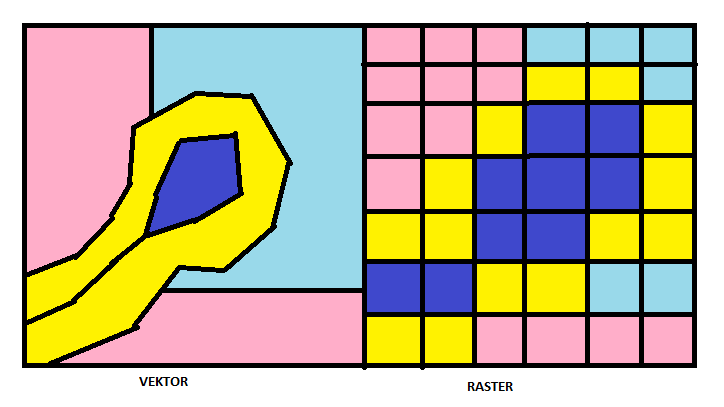
\includegraphics[width=1\textwidth]{figures/vektorraster.PNG}}
	\caption{Perbedaan Vektor dengan Raster.}
	\label{vektorraster}
	\end{figure}
Pada gambar \ref{vektorraster} merupakan contoh perbedaan antara vektor dengan raster.

\section{Tipe Data Vektor}
\subsection{Definisi Tipe Data Vektor}
Data vektor adalah data yang disimpan dalam bentuk koordinat titik yang menampilkan, 
menempatkan, dan menyimpan data spacial dengan menggunakan titik, garis atau polygon.
Terdapat tiga jenis tipe data vektor yaitu titik, garis, dan polygon. Tipe data ini 
biasanya terdapat pada peta. Setiap bagian dari data vektor bisa saja mempunyai 
informasi yang berasosiasi satu sama lain.
Model data vektor diwakili oleh simbol – simbol yang terdiri atas interkoneksi garis
dan titik yang merepresentasikan lokasi dan garis batas dari entitas geografi. Dalam
model data vektor , data dapat direpresentasikan sebagai Lines (garis), Polylines 
(polygon), Points (titik), Area (daerah), Nodes (titik potong) Pada model data vektor ini, 
suatu objek dinyatakan dalam bentuk koordinat(x,y) yang berhubungan satu sama lainnya kecuali objek titik.
\begin{figure}[ht]
	\centerline{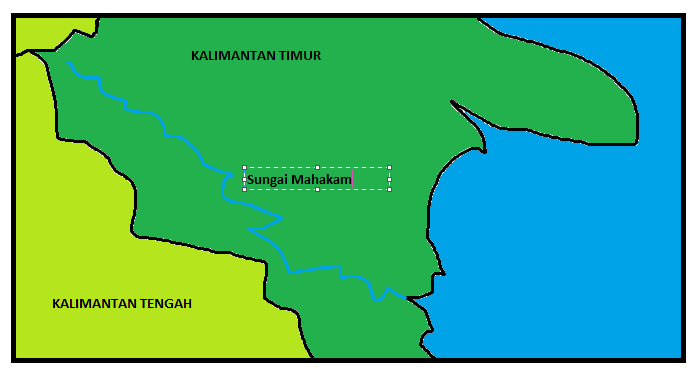
\includegraphics[width=1\textwidth]{figures/sungai.PNG}}
	\caption{Sungai merupakan contoh vektor line pada peta.}
	\label{sungai}
	\end{figure}
   
Pada gambar \ref{sungai} merupakan salah satu contoh data vektor line pada peta yaitu sungai.
\section{Data Atribut}
\subsection{pengertian Data Atribut}
Data atribut merupakan data yang mempresentasikan aspek-aspek deskripsi/penjelasan 
dari suatu fenomena di permukaan bumi dalam bentuk kata-kata, angka, atau tabel. 
Data atribut berfungsi untuk menggambarkan gejala topografi karena memiliki aspek deskriptif dan kualitatif. 
Oleh karena itu, data atribut sangat penting dalam menjelaskan seluruh objek geografi. 
Contohnya, atribut kualitas tanah terdiri atas status kepemilikian lahan, luas lahan, 
tingkat kesuburan tanah dan kandungan mineral dalam tanah. 
Data atribut bisa berupa data kuantitatif (angka) seperti data jumlah penduduk dan dapat berupa data kualitatif (mutu) 
seperti data tingkat kesuburan tanah.  
Bentuk-bentuk data atribut:
\begin{enumerate}
\item	Data kuantitatif (angka-angka/statistik), contoh: jumlah penduduk
\item	Data kualitatif (kualitas/mutu), contoh: tingkat kesuburan tanah
\end{enumerate}

\subsubsection{Kelebihan dan Kekurangan Data Atribut}
Kelebihan :
\begin{enumerate}
   \item Data dapat dimanipulasi 
   \item Dapat mengetahui jenis lokasi peta
\end{enumerate}
Kekurangan :
\begin{enumerate}
   \item Sulit membedakan gambar dan warna pada peta
   \item Sulit menentukan lokasi
\end{enumerate}

\section{Data Vektor Line}
\subsection{Pengertian}
  Line merupakan bahasa Inggris dari garis. Garis adalah bentuk geometri liniar yang
 menghubungkan dua titik atau lebih dan biasanya digunakan untuk mempresentasikan
 object berdimensi satu. batas object geometri polygon juga merupakan sebuah garis-garis,
 begitu pula dengan jaringan listrik, jaringan komunikasi, jaringan air minum, saluran buangan,
 dan utility lain yang dapat dipresentasikan sebagai object dengan bentuk geometri garis.
 Hal itu pula yang akan bergantung pada skala peta yang menjadi sumbernya atau skala
 representasi akhirnya.
  Garis bisa digunakan untuk menunjukkan route suatu perjalanan atau menggambarkan boundary. 
 Poligon bisa digunakan untuk menggambarkan sebuah danau atau sebuah Negara pada peta dunia. 
 Dalam format vektor, bumi direpresentasikan sebagai suatu mosaik dari garis (arc/line), 
 poligon (daerah yang dibatasi oleh garis yang berawal dan berakhir pada titik yang sama), 
 titik/ point (node yang mempunyai label), dan nodes (merupakan titik perpotongan antara dua baris).
  Seperti telah diuraikan sebelumnya, data vektor terbentuk dari tiga jenis geometri yakni 
 titik (point), garis (line), dan area (polygon). 
 Oleh karena itu, objek-objek di permukaan bumi perlu divisualisasikan 
 dalam ketiga geometri tersebut agar bisa diproses dengan GIS. 
 Contoh visualisasi dunia nyata menjadi elemen gambar ketiga geometri tersebut antara lain landmark dan fasilitas sebagai titik, 
 jalan dan sungai sebagai garis, dan daerah administrasi tertentu sebagai area. 
 Berikut ini penjelasan lebih dalam mengenai ketiga entitas geometri tersebut.
 
 \subsubsection{titik (point)}
  meliputi semua objek grafis atau geografis yang dikaitkan dengan pasangan koordinat (x,y). 
  Selain memuat informasi koordinat, data  titik juga bisa saja merupakan suatu simbol yang memiliki 
  keterkaitan dengan informasi lain.  Satu buah objek titik memiliki satu baris dalam tabel atribut. 
  Karakteristik-karakteristik dari titik ini dijelaskan oleh kolom-kolom yang dibentuk pada tabel atribut.
  
  \subsubsection{Garis (line)}
  merupakan semua unsur-unsur linier yang dibangun dengan menggunakan segmen-segmen garis lurus yang 
  dibentuk oleh dua titik koordinat atau lebih (Burrough, 1994). 
  Entitas garis yang paling sederhana memerlukan ruang untuk menyimpan titik awal dan titik akhir (dua pasangan koordinat x,y) 
  berserta informasi lain mengenai simbol yang digunakan untuk merepresentasikannya. 
  Garis tunggal yang terbentuk dari titik awal dan titik akhir saja disebut sebagai line. 
  Sedangkan garis bersegmen banyak yang terbentuk dari banyak titik (vertex) disebut polyline. 
  Dalam GIS, baik line maupun polyline dianggap sebagai suatu entitas yang sama yakni polyline. 
  Setiap satu entitas polyline memiliki satu baris dalam tabel atribut. 
  Karakteristik dari entitas ini disimpan dalam kolom-kolom tabel atribut. 
  
  \subsubsection{Area (polygon)}
  merupakan suatu objek tertutup yang memiliki luasan. Polygon dapat direpresentasikan dengan 
  berbagai cara di dalam model data vektor. Karena kebanyakan peta tematik yang digunakan dalam GIS berurusan dengan polygon,
  metode-metode representasi dan pemanipulasian entity ini banyak mendapat perhatian. 
  Seperti halnya titik dan polyline, satu objek poligon juga diwakili oleh satu baris pada tabel atribut. 
  Poligon biasanya digunakan untuk merepresentasikan objek dunia nyata yang memiliki luasan seperti 
  wilayah administrasi, danau, guna lahan, jenis tanah, dan sebagainya
 
 \subsubsection{Kelebihan dan Kekurangan Data Vektor Line}
 Kelebihan:
 \begin{enumerate}
    \item Memerlukan ruang atau tempat menyimpan yang lebih sedikit di computer.
    \item Satu layer dapat dikaitkan dengan atau mengunakan atribut sehingga dapat menghemat ruang penyimpanan secara keseluruhan.
    \item Dengan banyak atribut yang banyak dikandung oleh satu layer, 
             banyak peta tematik lain yang dapat dihasilkan sebagai peta turunannya.
    \item Hubungan topologi dan network dapat dilakukan dengan mudah.
    \item Memiliki resolusi spasial yang tinggi.
    \item Representasi grafis data spasialnya sangat mirip dengan peta garis buatan tangan manusia.
    \item Memiliki batas-batas yang teliti, tegas dan jelas sehingga sangat baik untuk 
    pembuatan peta-peta administrasi dan persil tanah milik.
    \item Transformasi koordinat dan proyeksi tidak sulit dilakukan. 
 \end{enumerate}
 Kekurangan:
 \begin{enumerate}
    \item Memiliki struktur data yang kompleks.
    \item Datanya tidak mudah untuk dimanipulasi.
    \item Pengguna tidak mudah berkreasi untuk membuat programnya sendiri untuk memenuhi kebutuhan aplikasinya. 
             Hal ini disebabkan oleh struktur data vector yang lebih kompleks dan prosedur fungsi dan analisisnya 
             memerlukan kemampuan tinggi karena lebih sulit. 
            Pengguna harus membeli system perangkat lunaknya karena teknologinya masih mahal. Prosedurnyapun terkadang lebih sulit.
    \item Karena proses keseluruhan untuk mendapatkannya lebih lama, peta vector seringkali mengalami out of date atau kadaluarsa.
    \item Memerlukan perangkat keras dan perangkat lunak yang lebih mahal.
    \item Overlay beberapa layers vector secara simultan memerlukan waktu yang relative lama.
 \end{enumerate}
 
 \section{Raster}
 \subsection{Pengertian Raster}
Data raster (juga dikenal sebagai data grid) mewakili tipe keempat dari fitur: permukaan. 
Data raster berbasis sel dan kategori data ini juga mencakup citra udara dan satelit. 
Ada dua jenis data raster: kontinu dan diskrit. Contoh data raster diskrit adalah kepadatan penduduk. 
Contoh data kontinyu adalah pengukuran suhu dan elevasi. Ada juga tiga jenis dataset raster: data tematik, 
data spektral, dan gambar.Raster dataset adalah intrinsik untuk analisis spasial yang paling. 
Analisis data seperti ekstraksi kemiringan dan aspek dari Digital Elevation Models terjadi dengan dataset raster.
Pemodelan hidrologi spasial seperti ekstraksi daerah aliran sungai dan jalur aliran juga menggunakan sistem berbasis raster.
Data spektral menyajikan citra udara atau satelit yang kemudian sering digunakan 
untuk memperoleh informasi geologi vegetasi dengan mengklasifikasikan tanda tangan spektral dari setiap jenis fitur.

\subsubsection{Karakteristik Raster}
Resolusi suatu data raster akan merujuk pada ukunan permukaan bumi yang direpresentasikan oleh setiap piksel. 
Makin kecil ukuran atau luas permukaan bumi yang dapat direpresentasikan oleh setiap pikselnya, makin tinggi resolusi spasialnya.
Piksel-piksel di dalam zone atau area yang sejenis memiliki nilai (isi piksel atau ID number) yang sama.
Pada umumnya, lokasi di dalam model data raster, diidentifikasi dengan menggunakan pasangan koordinat kolom dan baris (x,y).
Nilai yang merepresentasikan suatu piksel dapat dihasilkan dengan cara sampling yang berlainan:
\begin{enumerate}
\item Nilai suatu piksel merupakan nilai rata-rata sampling untuk wilayah yang direpresentasikannya.
\item Nilai suatu piksel adatah nilai sampling yang berposisi di pusat (atau di tengah) piksel yang bersangkutan.
\item Nilai suatu pikset adatah nilai sample yang tertetak di sudut-sudut grid.
\end{enumerate}

\subsubsection{Kelebihan dan Kekurangan Raster}
 Kelebihan :
 \begin{enumerate}
    \item Memiliki struktur data yang sederhana
    \item Mudah dimanipulasi dengan menggunakan fungsi-fungsi matematis sederhana
    \item Teknologi yang digunakan cukup murah dan tidak begitu kompleks sehingga pengguna dapat 
             membuat sendiri program aplikasi yang mengunakan citra raster.
    \item Compatible dengan citra-citra satelit penginderaan jauh dan semua image hasil scanning data spasial.
    \item Overlay dan kombinasi data raster dengan data inderaja mudah dilakukan
    \item Memiliki kemampuan-kemampuan permodelan dan analisis spasial tingkat lanjut
    \item Metode untuk mendapatkan citra raster lebih mudah
    \item Gambarab permukaan bumi dalam bentuk citra raster yang didapat dari radar atau satelit 
             penginderaan jauh selalu lebih actual dari pada bentuk vektornya
    \item Prosedur untuk memperoleh data dalam bentuk raster lebih mudah, sederhana dan murah.
    \item Harga system perangkat lunak aplikasinya cenderung lebih murah.
 \end{enumerate}
 Kekurangan:
 \begin{enumerate}
    \item Secara umum memerlukan ruang atau tempat menyimpan (disk) yang besar dalam computer, 
             banyak terjadi redudacy data baik untuk setiap layer-nya maupun secara keseluruhan.
    \item Penggunaan sel atau ukuran grid yang lebiih besar untuk menghemat ruang penyimpanan akan 
             menyebabkan kehilangan informasi dan ketelitian.
    \item Sebuah citra raster hanya mengandung satu tematik saja sehingga sulit digabungkan 
             dengan atribut-atribut lainnya dalam satu layer.
    \item Tampilan atau representasi dan akurasi posisi sangat bergantung pada ukuran pikselnya (resolusi spasial).
    \item Sering mengalami kesalahan dalam menggambarkan bentuk dan garis batas suatu objek, 
             sangat bergantung pada resolusi spasial dan toleransi yang diberikan.
    \item Transformasi koordinat dan proyeksi lebih sulit dilakukan
    \item Sangat sulit untuk merepresentasikan hubungan topologi (juga network).
    \item Metode untuk mendapatkan format data vector melalui proses yang lama, cukup melelahkan dan relative mahal.
  \end{enumerate}
